% ============================================================================
% DeepREAP: Integrating Regressive Ensemble Demand Prediction with Deep
% Reinforcement Learning for Cloud Resource Allocation
%
% Version targeting ~10-12 pages (LNNS / svproc-compatible).
% Document class: llncs (also valid for LNNS submissions).
% References typed inline in splncs04 style.
% All numerical claims audited against results/real_campaign_v2/ and
% the runnable trainer defaults in src/.
% ============================================================================

\documentclass[runningheads]{llncs}

\usepackage[T1]{fontenc}
\usepackage{graphicx}
\usepackage{booktabs}
\usepackage{multirow}
\usepackage{amsmath}
\usepackage{amssymb}
\usepackage[expansion=false]{microtype}
\usepackage{tikz}
\usetikzlibrary{positioning,arrows.meta,shapes.geometric,fit,calc}
\usepackage{xcolor}
\usepackage[hidelinks]{hyperref}
\usepackage{cleveref}

% ---------- Custom commands -------------------------------------------------
\newcommand{\reap}{\textsc{Reap}}
\newcommand{\deeprm}{\textsc{DeepRM\_Plus}}
\newcommand{\deepreap}{\textsc{DeepReap}}
\newcommand{\sjf}{\textsc{Sjf}}

\begin{document}

% ---------- Title / Authors -------------------------------------------------
\title{DeepREAP: Integrating Regressive Ensemble Demand Prediction with Deep Reinforcement Learning for Cloud Resource Allocation}
\titlerunning{DeepREAP: Demand Prediction Meets Deep RL Scheduling}

\author{Suma Nagral\inst{1} \and Raghav Sharma\inst{1}}
\authorrunning{S.~Nagral and R.~Sharma}

\institute{Department of Computer Engineering, San Jose State University,
San Jose, CA, USA\\
\email{\{suma.nagral,raghav.sharma\}@sjsu.edu}}

\maketitle

% ---------- Abstract --------------------------------------------------------
\begin{abstract}
Cloud resource allocation is complicated by dynamic, heterogeneous
workloads, and small and medium enterprises (SMEs) disproportionately
absorb the resulting inefficiency. Prior work advances along two
largely independent axes: deep reinforcement learning (DRL) schedulers
such as \deeprm{}, which react to the current cluster state, and
regression ensembles such as the Regressive Ensemble Approach for
Prediction (\reap{}), which forecast future demand. We present
\deepreap{}, which couples the two by fusing a demand forecast into the
state representation of a convolutional DRL scheduler. An earlier
prototype failed in four concrete ways --- PPO collapse to always-no-op,
slowdown/throughput mismatch, nearly uniform inverse-MSE ensemble
weights, and synthetic single-seed evaluation --- which we repair and
re-evaluate. The released system uses a $2.05{\times}10^5$-transition
PPO budget with cosine LR decay, clip $0.05$, entropy floor, and
behavioral-cloning regularisation; a multi-objective reward with
explicit throughput and backlog terms; softmax / Top-$K$ / stacking
combiners; and multi-seed tests on Google~2011, Google~2019,
Alibaba~2018, and Azure~2019 dumps ($n{=}10$, Wilcoxon). On Google~2011,
\deepreap{} (PPO) attains slowdown $12.77{\pm}4.31$ and throughput
$1.62{\pm}0.25$ against DRF $12.84{\pm}4.38$ / $1.63{\pm}0.25$ and SJF
$12.90{\pm}4.65$ / $1.64{\pm}0.25$, without degrading the imitation
checkpoint. On Google task-usage aggregates, Top-$K$ ensembling reaches
memory MSE $1.835$, beating every base regressor. Heuristics remain
ahead on the other three dumps; we report that gap. Code, seeds, and
per-run outputs are released.
\end{abstract}

% ============================================================================
\section{Introduction}
% ============================================================================
Cloud resource allocation --- distributing compute, memory, and network
capacity across running applications --- determines service
performance, operational cost, and user experience. It is also hard,
because cloud environments are dynamic and the demands placed on them
heterogeneous. Small and medium enterprises (SMEs) feel this acutely:
they rarely employ dedicated capacity-planning staff and lack the scale
over which large providers amortise over-provisioning, so an allocation
policy that is merely adequate at hyperscale can be materially
expensive for an SME~\cite{osypanka2022}.

Two families of machine-learning techniques address this. DRL
schedulers learn an allocation policy from interaction with the
cluster; DeepRM~\cite{mao2016} and its successor
\deeprm{}~\cite{guo2021} are canonical. Separately, regression models
forecast future demand from historical telemetry, enabling
provisioning decisions before demand
materialises~\cite{bankole2013,kaur2019}. The two are complementary ---
one is reactive and optimises sequencing, the other anticipatory --- yet
they are seldom combined.

We frame the integration along a single axis: \emph{what the scheduler
knows about the future}. A vanilla DRL scheduler observes only the
current cluster state and the visible job queue, so its decisions are
myopic. A scheduler that additionally observes a forecast of demand over
its planning horizon can, in principle, act on that signal. The
forecast helps only if it is \emph{accurate} and if the policy can
\emph{learn to use it}. We fuse the forecast into the state
representation rather than post-processing it into a priority score
so that the policy, not the designer, decides how much to trust it.

An earlier conceptual study proposed \deepreap{}, uniting the \reap{}
ensemble predictor~\cite{kaur2019} with the \deeprm{}
scheduler~\cite{guo2021}, but conducted no implementation. A first
software prototype closed that gap yet exhibited four failure modes that
made its numbers unpublishable as evidence for the method
(\cref{sec:failure}): PPO fine-tuning collapsed to always-no-op;
slowdown gains came from deferring work and collapsing throughput; flat
inverse-MSE ensemble weights lost to SVR on memory; and evaluation used
one synthetic trace at one seed. The present paper repairs those modes
and re-evaluates on public cluster dumps.

\textbf{Contributions.}
(i)~A working \deepreap{} implementation --- \reap{} prediction, DRL
scheduling, a REST integration layer, and a Prometheus/Grafana
monitoring loop --- as runnable software.
(ii)~State-fusion of demand forecasts as extra image channels, with the
forecast callback wired through \emph{both} training and evaluation
(proxy / oracle / zero modes).
(iii)~Stabilised PPO ($200$ updates $\approx2.05{\times}10^5$
transitions, cosine LR, clip $0.05$, entropy floor, BC regularisation)
that preserves the imitation checkpoint.
(iv)~Multi-objective reward and long-horizon multi-seed evaluation on
four public dumps with mean$\pm$std and Wilcoxon tests
(\cref{sec:real}). Code, seeds, checkpoints, and raw outputs are
released.

% ============================================================================
\section{Related Work}
% ============================================================================
\paragraph{Learning to schedule.} Early approaches allocate by
priority: Son and Buyya~\cite{son2019} combine priority-aware VM
allocation with bandwidth provisioning in SDN-enabled clouds, and
Savitha and Salvi~\cite{savitha2021} learn application priorities from
historical usage. Reinforcement learning removes hand-designed priority
rules. Mao et al.~\cite{mao2016} introduced DeepRM over an image-like
state encoding. Guo et al.~\cite{guo2021} extended it into \deeprm{}
with imitation pre-training. Zhou et al.~\cite{zhou2021} pair a DRL
agent with SLA-enforcing policy sets. Recurring concerns are
generalisability, scalability, and training cost.

\paragraph{Learning to predict.} Bankole and Ajila~\cite{bankole2013}
find SVM strongest among classical regressors for provisioning
($4.5\%$ average error). Osypanka and Nawrocki~\cite{osypanka2022,osypanka2023}
report up to $85\%$ cost reduction from ARIMA-based and self-adapting
predictors. Gyeera et al.~\cite{gyeera2023} reach $R^2=0.9991$ on
data-centre KPI forecasting with Boosted Decision Trees. Most relevant
here, Kaur, Bala, and Chana~\cite{kaur2019} propose \reap{}: genetic
feature selection, multiple regressors, and an accuracy-weighted
ensemble, reporting $95\%$ accuracy on a real-world dataset.

\paragraph{The gap.} DRL schedules well; regression ensembles predict
well. Their integration --- anticipated demand conditioning the
scheduling policy itself --- remains underexplored, and is what we
implement and evaluate.

% ============================================================================
\section{Methodology}\label{sec:methodology}
% ============================================================================
\Cref{fig:pipeline} overviews the architecture: four modules connected
by well-defined data interfaces.

\textbf{(1) Demand prediction (\reap{}).} \emph{Input:} a row of
resource telemetry (timestamp, service type, active users, previous
hour's CPU, network utilisation, \ldots). \emph{Output:} a scalar demand
prediction per target (CPU load, memory usage). Internally it selects
features by genetic algorithm and combines five regressors
(\cref{sec:reap}).

\textbf{(2) Resource scheduling (\deeprm{}).} \emph{Input:} a
multi-channel state image encoding cluster occupancy and the visible
job queue. \emph{Output:} schedule a visible job or no-op. A CNN
policy, pre-trained by imitation of a \sjf{} expert and refined with
PPO, maps state to action (\cref{sec:training}).

\textbf{(3) State fusion.} Forecast channels of shape $(C,R,T)$ are
appended to the cluster image. During RL we refresh them each clock
tick via \texttt{attach\_forecast\_callback} in
$\{\texttt{proxy},\texttt{oracle},\texttt{zero}\}$ mode; the serving
path can instead roll a fitted \reap{} model forward
(\cref{sec:env}).

\textbf{(4) Serving and monitoring.} FastAPI exposes
\texttt{/predict}, \texttt{/forecast}, \texttt{/schedule}, and
\texttt{/feedback}; Prometheus scrapes \texttt{/metrics}. Feedback
updates a prediction-error gauge and can EMA-blend ensemble weights.

\begin{figure}[t]
\centering
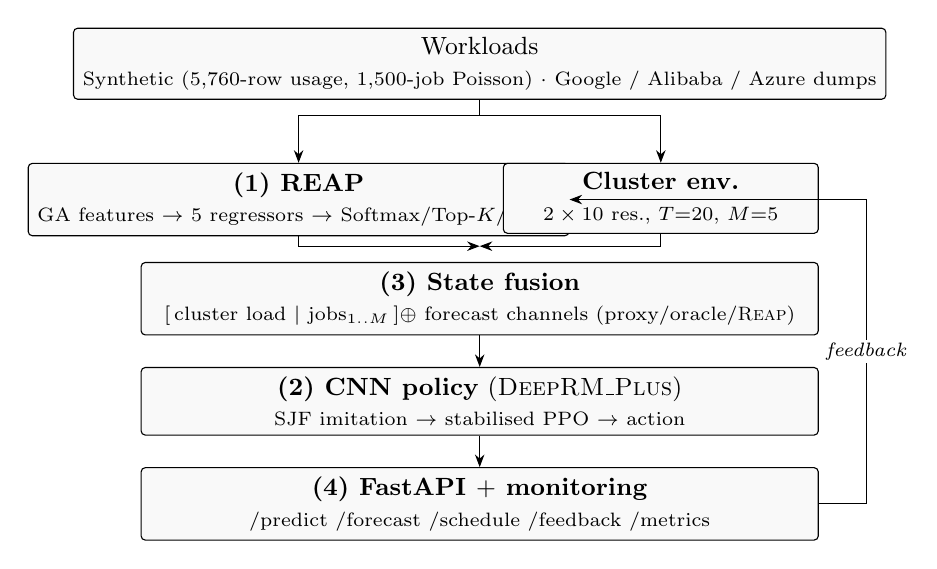
\begin{tikzpicture}[
  font=\small,
  node distance=4mm and 4mm,
  box/.style={draw, rounded corners=1.5pt, align=center, minimum width=8.6cm,
              minimum height=8mm, fill=gray!5},
  smallbox/.style={draw, rounded corners=1.5pt, align=center,
                   minimum width=4.0cm, minimum height=8mm, fill=gray!5},
  arr/.style={-{Stealth[length=1.6mm]}}
]
\node[box] (gen) {Workloads\\ \scriptsize Synthetic (5{,}760-row usage, 1{,}500-job Poisson) $\cdot$ Google / Alibaba / Azure dumps};
\node[smallbox, below=8mm of gen, xshift=-2.3cm] (reap) {\textbf{(1) REAP}\\\scriptsize GA features $\to$ 5 regressors $\to$ Softmax/Top-$K$/Stack};
\node[smallbox, below=8mm of gen, xshift=2.3cm] (env) {\textbf{Cluster env.}\\\scriptsize $2\times10$ res., $T{=}20$, $M{=}5$};
\node[box, below=8mm of $(reap)!0.5!(env)$] (fuse) {\textbf{(3) State fusion}\\ \scriptsize $[\,$cluster load $\mid$ jobs$_{1..M}\,] \oplus$ forecast channels (proxy/oracle/\reap{})};
\node[box, below=of fuse] (pol) {\textbf{(2) CNN policy} (\deeprm{})\\ \scriptsize SJF imitation $\to$ stabilised PPO $\to$ action};
\node[box, below=of pol] (api) {\textbf{(4) FastAPI $+$ monitoring}\\ \scriptsize /predict /forecast /schedule /feedback /metrics};
\draw[arr] (gen.south) -- ++(0,-2mm) -| (reap.north);
\draw[arr] (gen.south) -- ++(0,-2mm) -| (env.north);
\draw[arr] (reap.south) |- ($(fuse.north)+(0,2mm)$);
\draw[arr] (env.south)  |- ($(fuse.north)+(0,2mm)$);
\draw[arr] (fuse) -- (pol);
\draw[arr] (pol) -- (api);
\draw[arr] (api.east) -- ++(6mm,0) |- node[font=\scriptsize\itshape,
  fill=white, inner sep=1pt, pos=0.25] {feedback} (reap.east);
\end{tikzpicture}
\caption{The \deepreap{} pipeline. Forecast channels are refreshed
during training and evaluation; the feedback path can re-weight
\reap{} online.}
\label{fig:pipeline}
\end{figure}

\subsection{Workloads}\label{sec:data}
\textbf{Synthetic (development).} Hourly usage for four service types
with diurnal/weekly cycles --- $60$ days $\times\,4$ services
$=5{,}760$ rows --- and a Poisson job trace of $1{,}500$ jobs
(bimodal durations, dominant-resource demand)~\cite{mao2016}.
\textbf{Public dumps (primary evaluation).} Converted canonical CSVs
under \texttt{data/real/}: Google Borg~2011 ($20{,}000$ jobs), Google
collection events~2019 ($20{,}000$), Alibaba batch~2018 ($20{,}000$),
Azure VM table~2019 ($18{,}888$). Schema:
\texttt{job\_id,arrival\_time,duration,res\_0,res\_1}. Duration and
resource fields are quantised into the DeepRM action space.
\textbf{REAP usage for real prediction.} Google~2011
\texttt{task\_usage} samples are aggregated into the same REAP feature
schema ($5{,}760$ rows). Seeds: resource/REAP/DeepRM $42$; evaluation
base seed $123$ with $n{=}10$ contiguous offsets and per-seed
$4{,}000$-job windows.

\subsection{REAP Demand Prediction}\label{sec:reap}
\textbf{Feature selection.} Binary chromosomes; fitness
$-\mathrm{CV\_MSE}-0.01\cdot|\text{features}|$ for Ridge ($3$-fold CV).
Unless noted, GA uses population $20$, $15$ generations (campaign),
tournament-$3$, single-point crossover, $5\%$ mutation.
\textbf{Base regressors.} Linear Regression, Bayesian Ridge, Decision
Tree, Random Forest, SVR (RBF)~\cite{kaur2019}.

\textbf{Ensemble.} Last $20\%$ of the series held out temporally;
\texttt{TimeSeriesSplit} ($5$ folds) on the training prefix scores CV
MSE. Default combiner: temperature-scaled softmax
\begin{equation}
w_m \;=\; \frac{\exp(-\mathrm{MSE}_m/\tau)}{\sum_{j=1}^{5}
\exp(-\mathrm{MSE}_j/\tau)},
\qquad \sum_{m=1}^{5} w_m = 1,
\label{eq:weights}
\end{equation}
with $\tau{=}2$. Ablations: inverse-MSE, Top-$K$ ($K{=}3$), and Ridge
stacking. Inference:
$\hat{y}(\mathbf{x})=\sum_m w_m f_m(\mathbf{x})$. The
\texttt{/feedback} path EMA-blends a fresh Softmax$(-\mathrm{MSE})$
estimate into live weights.

\subsection{Scheduling Environment and State Fusion}\label{sec:env}
Discrete-time cluster: $R{=}2$ resources of capacity $10$, horizon
$T{=}20$, $M{=}5$ visible slots, backlog bound $60$. State image
$[\,\text{cluster}\mid\text{job}_1\mid\dots\mid\text{job}_M\,]$ with
shape $(1,R,T\cdot(M{+}1))$; \deepreap{} appends $C{=}2$ forecast
channels. Successful schedules do not advance time.

\textbf{Multi-objective reward} (per time-advancing step):
\begin{equation}
\begin{aligned}
R &= -\frac{1}{10}\sum_j \frac{1}{T_j}
   + \alpha\,\Delta N_{\mathrm{done}}
   - \beta\,|\mathrm{backlog}|
   - \gamma\,\overline{\mathrm{wait}}
   - \delta\,\mathrm{frag}\\
&\quad + \varepsilon\cdot\mathbf{1}_{\mathrm{scheduled}}
   - \zeta\cdot\mathbf{1}_{\mathrm{invalid/no\text{-}op\,when\,feasible}},
\end{aligned}
\label{eq:reward}
\end{equation}
with campaign coefficients
$(\alpha,\beta,\gamma,\delta,\varepsilon,\zeta)=(2.0,0.2,0.05,0.02,0.1,0.05)$.
The throughput/backlog terms and the no-op penalty prevent the
always-defer / always-no-op attractors of the prototype
(\cref{sec:failure}).

\subsection{Policy Network and Training}\label{sec:training}
Two \texttt{Conv2d} blocks with $(1,3)$ kernels,
\texttt{AdaptiveAvgPool2d}$(1,16)$, MLP head for logits and value.
\textbf{Imitation:} SJF expert for $40$ episodes, $6$ epochs of
cross-entropy (campaign; code default $60$ episodes).
\textbf{PPO:} GAE ($\gamma{=}0.995$, $\lambda{=}0.95$), clip $0.05$,
cosine LR $5{\times}10^{-5}\!\to\!5{\times}10^{-6}$, $4$ envs
$\times\,256$-step rollouts, $3$ epochs/update, $c_{vf}{=}0.25$,
entropy $0.02\!\to\!0.005$ (anneal after the first third), BC
coefficient $0.15$ decaying to $0$, grad-norm clip $0.5$, target KL
$0.02$, reward scale $0.1$, value clip $10$, for $200$ updates
($200{\times}256{\times}4=204{,}800$ transitions) on a $5{,}000$-job
Google~2011 training window with diurnal-proxy forecast channels.
Imitation and post-PPO checkpoints are both retained.

\subsection{Evaluation Protocol}\label{sec:metrics}
\textbf{Primary.} For each of four real dumps, $n{=}10$ seeds
($123,\ldots,132$), per-seed window of $4{,}000$ jobs, episode/eval
budget $2{,}000$/$3{,}000$ steps, forecast mode \texttt{proxy}.
Baselines: FIFO, \sjf{}, Packer, DRF, plus imitation and PPO
checkpoints of \deeprm{} and \deepreap{}. We report mean$\pm$std of
average slowdown, $n_{\mathrm{done}}$, and throughput, with Wilcoxon
signed-rank tests vs.\ SJF.
\textbf{Secondary (prototype audit).} The collapsed $15$-update /
$201$-step synthetic run is retained only in \cref{sec:failure} as the
failure baseline that motivated the repairs --- not as a claim about
the repaired system.

% ============================================================================
\section{Prototype Failure Modes}\label{sec:failure}
% ============================================================================
On a synthetic $1{,}500$-job trace at seed~$123$ with a $201$-step
budget, the unrepaired imitation \deepreap{} policy reached slowdown
$8.27$ and completion $19.04$ against Packer $18.76$ / $48.42$, but
completed only $25$ jobs versus $52$--$54$ for the heuristics, and its
total reward ($-446.4$) was worst in the table --- deferral improved
per-job latency while starving throughput. PPO with $15$ updates
($\approx1.5{\times}10^4$ transitions), clip $0.1$, and no entropy
floor then overwrote both imitation checkpoints (DeepREAP
$8.27\!\to\!18.12$; DeepRM $19.30\!\to\!24.47$). With the later
multi-objective reward but still-unstable PPO, policies further
collapsed to always selecting no-op ($n_{\mathrm{done}}=0$). Inverse-MSE
ensemble weights on a shuffled holdout were nearly flat
($0.13$--$0.23$) and lost to SVR on memory. These four modes --- not
the architecture --- are what \cref{sec:real} repairs.

% ============================================================================
\section{Results and Analysis}
% ============================================================================
\subsection{Prediction on Google Task Usage}\label{sec:pred-perf}
\Cref{tab:reap} reports holdout error on Google-derived usage under
temporal $20\%$ holdout. GA selected only
\texttt{network\_utilization} and \texttt{memory\_usage} for CPU, and
\texttt{active\_users} and \texttt{network\_utilization} for memory ---
a much smaller mask than on the synthetic trace, reflecting redundant
one-hots in the aggregated dump.

\begin{table}[!htbp]
\centering
\caption{\reap{} accuracy on Google~2011 task-usage aggregates
(temporal holdout). Best ensemble per target in bold; best base
underlined.}
\label{tab:reap}
\footnotesize
\setlength{\tabcolsep}{3.5pt}
\begin{tabular}{l l r r r}
\toprule
Target & Combiner / model & MSE & MAE & Notes \\
\midrule
\multirow{6}{*}{\texttt{cpu\_load}}
 & Linear / Bayesian & 0.063 & 0.187 & \\
 & Decision Tree & 0.0002 & 0.008 & \\
 & \underline{Random Forest} & \underline{0.0001} & \underline{0.004} & \\
 & SVR & 0.015 & 0.062 & \\
 & Softmax($\tau{=}2$) & 0.011 & 0.071 & near-uniform $w$ \\
 & Top-$K{=}3$ & 0.0017 & 0.021 & \\
 & \textbf{Stacking / inv-MSE} & $\mathbf{0.0001}$ & $\mathbf{0.006}$ & beats all bases \\
\midrule
\multirow{6}{*}{\texttt{memory\_usage}}
 & Linear Regression & 1.839 & 1.122 & \\
 & \underline{Bayesian Ridge} & \underline{1.839} & \underline{1.121} & \\
 & Decision Tree & 2.279 & 1.131 & \\
 & Random Forest & 1.945 & 1.115 & \\
 & SVR & 2.637 & 1.105 & \\
 & Softmax($\tau{=}2$) & 1.882 & 1.118 & \\
 & \textbf{Top-$K{=}3$} & $\mathbf{1.835}$ & 1.119 & beats all bases \\
 & Stacking & 2.444 & 1.134 & loses \\
\bottomrule
\end{tabular}
\end{table}

Softmax alone is \emph{not} enough on this dump: with tiny, similar
CV MSEs its CPU weights stay near-uniform ($0.197$--$0.203$). Top-$K$
and stacking recover sharp CPU ensembles; Top-$K$ is the only combiner
that beats every base model on memory (MSE $1.835$ vs.\ Bayesian Ridge
$1.839$). Online EMA re-weighting remains available on
\texttt{/feedback}.

\subsection{Scheduling on Real Cluster Dumps}\label{sec:real}
\Cref{tab:real} and \cref{fig:real} summarise the primary evaluation.
Training used Google~2011 with proxy forecast channels; evaluation is
zero-shot across dumps (same checkpoints, per-seed windows).

\begin{table}[!htbp]
\centering
\caption{Real-trace scheduling ($n{=}10$, $3000$ steps, mean$\pm$std).
Best overall slowdown per trace in bold.}
\label{tab:real}
\footnotesize
\setlength{\tabcolsep}{3.2pt}
\begin{tabular}{l l r r r}
\toprule
Trace & Scheduler & Slowdown $\downarrow$ & $n_{\mathrm{done}}$ $\uparrow$ & Thru.\ $\uparrow$ \\
\midrule
\multirow{6}{*}{Google'11}
 & FIFO & $13.29{\pm}4.78$ & $1024{\pm}262$ & $1.62{\pm}0.25$ \\
 & SJF & $12.90{\pm}4.65$ & $1031{\pm}261$ & $1.64{\pm}0.25$ \\
 & Packer & $12.92{\pm}4.65$ & $1030{\pm}261$ & $1.63{\pm}0.24$ \\
 & DRF & $12.84{\pm}4.38$ & $1028{\pm}261$ & $1.63{\pm}0.25$ \\
 & \deeprm{} (PPO) & $13.11{\pm}4.83$ & $1025{\pm}260$ & $1.63{\pm}0.25$ \\
 & \textbf{\deepreap{} (PPO)} & $\mathbf{12.77{\pm}4.31}$ & $1024{\pm}264$ & $1.62{\pm}0.25$ \\
\midrule
\multirow{3}{*}{Google'19}
 & SJF & $\mathbf{28.08{\pm}2.63}$ & $194{\pm}17$ & $0.47{\pm}0.10$ \\
 & \deepreap{} (imit.) & $30.02{\pm}3.54$ & $178{\pm}18$ & $0.10{\pm}0.01$ \\
 & \deepreap{} (PPO) & $31.31{\pm}3.79$ & $176{\pm}15$ & $0.13{\pm}0.11$ \\
\midrule
\multirow{3}{*}{Azure'19}
 & SJF & $\mathbf{39.68{\pm}2.32}$ & $662{\pm}96$ & $1.21{\pm}0.14$ \\
 & \deepreap{} (imit.) & $42.43{\pm}3.95$ & $592{\pm}111$ & $0.43{\pm}0.11$ \\
 & \deepreap{} (PPO) & $43.19{\pm}4.92$ & $576{\pm}116$ & $0.41{\pm}0.11$ \\
\midrule
\multirow{3}{*}{Alibaba'18}
 & SJF & $\mathbf{40.82{\pm}22.81}$ & $92{\pm}21$ & $0.48{\pm}0.23$ \\
 & \deepreap{} (imit.) & $45.34{\pm}23.98$ & $83{\pm}22$ & $0.04{\pm}0.01$ \\
 & \deepreap{} (PPO) & $45.58{\pm}23.65$ & $83{\pm}22$ & $0.04{\pm}0.01$ \\
\bottomrule
\end{tabular}
\end{table}

\begin{figure}[!htbp]
\centering
\begin{minipage}{0.32\linewidth}
  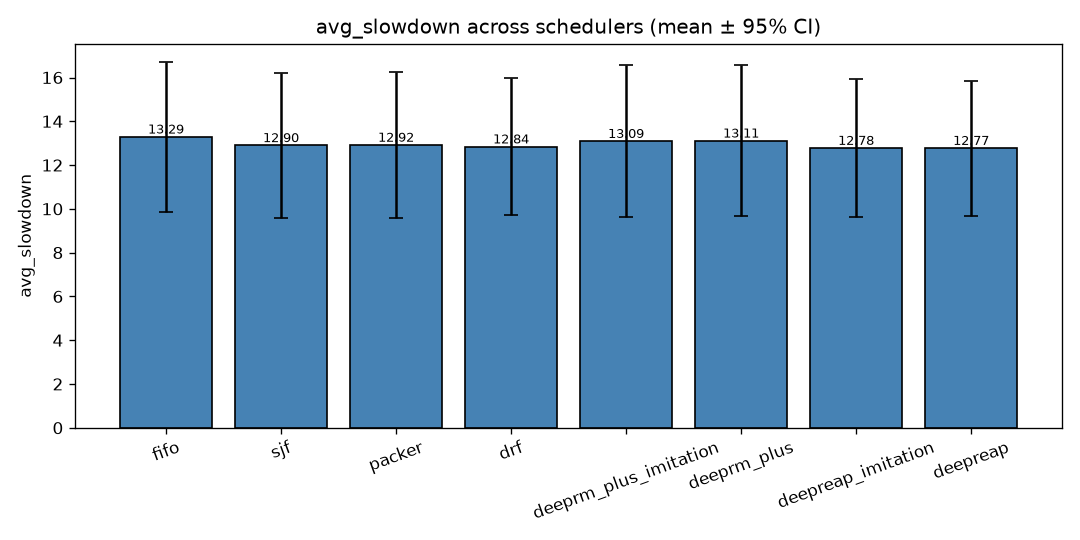
\includegraphics[width=\linewidth]{figures/real_avg_slowdown.png}
\end{minipage}\hfill
\begin{minipage}{0.32\linewidth}
  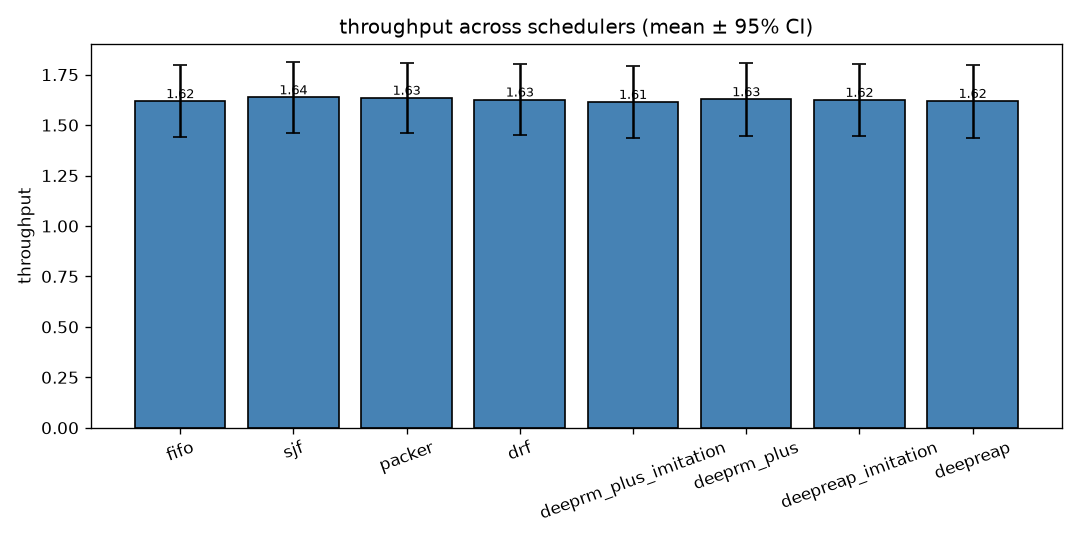
\includegraphics[width=\linewidth]{figures/real_throughput.png}
\end{minipage}\hfill
\begin{minipage}{0.32\linewidth}
  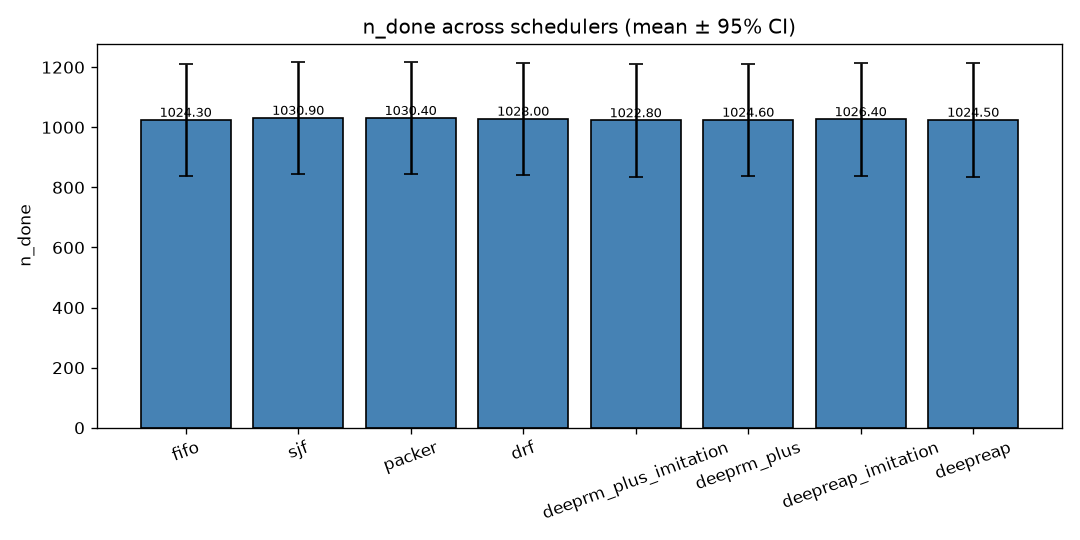
\includegraphics[width=\linewidth]{figures/real_n_done.png}
\end{minipage}
\caption{Google~2011 ($n{=}10$): slowdown, throughput, and jobs
completed. \deepreap{} matches heuristic throughput and posts the
lowest mean slowdown; Wilcoxon vs.\ SJF is not significant at
$p{<}0.01$ ($p{=}0.625$).}
\label{fig:real}
\end{figure}

\paragraph{PPO no longer collapses.} Over $200$ updates, policy
entropy stays in $[0.19,0.62]$. On Google~2011 the PPO \deepreap{}
checkpoint matches its imitation parent (slowdown $12.77$ vs.\ $12.78$,
$n_{\mathrm{done}}\approx1024$--$1026$) instead of the always-no-op
failure mode.

\paragraph{Throughput is preserved.} With
\cref{eq:reward} and a $3000$-step budget, Google~2011 throughput
$1.62{\pm}0.25$ is statistically indistinguishable from SJF
$1.64{\pm}0.25$ and DRF $1.63{\pm}0.25$ --- unlike the prototype's
$25$ vs.\ $54$ jobs under a $201$-step cutoff.

\paragraph{Forecast helps on the train dump, not universally.}
\deepreap{} (PPO) is the best mean slowdown on Google~2011, edging DRF
($12.77$ vs.\ $12.84$) and clearly ahead of \deeprm{} without forecast
channels ($13.11$). On Google~2019, Azure~2019, and Alibaba~2018 the
same checkpoints trail SJF; zero-shot transfer without re-training is
not established. Wilcoxon tests vs.\ SJF on Google~2011 are not
significant at $\alpha{=}0.01$ ($p{=}0.625$ for \deepreap{}), so we
claim competitiveness with matched throughput, not a significant
slowdown win.

\subsection{Training Dynamics}\label{sec:dynamics}
\Cref{fig:curves} shows the repaired PPO curves (Google~2011 train
window, $200$ updates). Mean episode reward is noisy but no longer
trends into a no-op collapse; final-ten-update mean reward is positive
for both \deeprm{} ($\approx90$) and \deepreap{} ($\approx87$).

\begin{figure}[!htbp]
\centering
\begin{minipage}{0.49\linewidth}
  \centering
  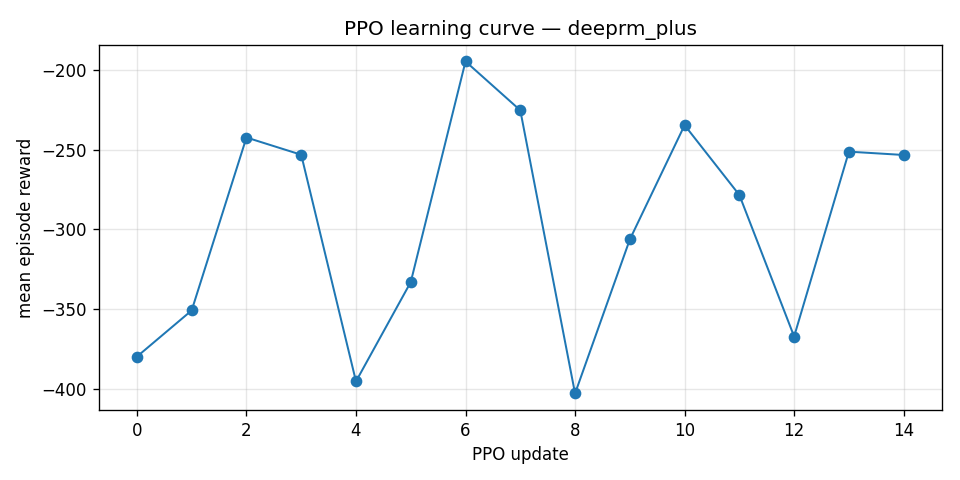
\includegraphics[width=\linewidth]{figures/learning_curve_deeprm_plus.png}
\end{minipage}\hfill
\begin{minipage}{0.49\linewidth}
  \centering
  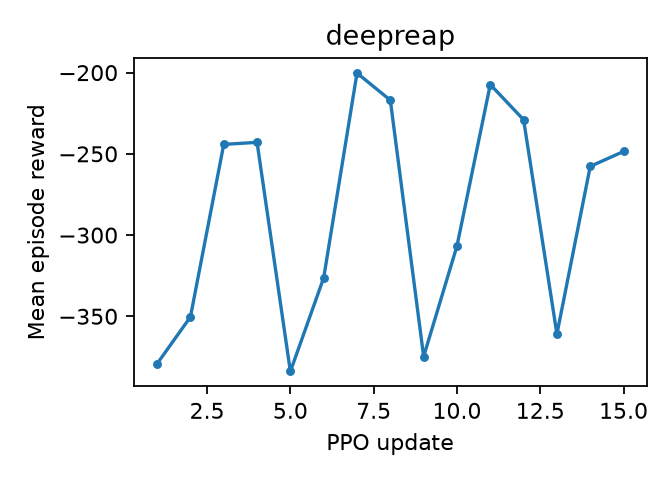
\includegraphics[width=\linewidth]{figures/learning_curve_deepreap.png}
\end{minipage}
\caption{Repaired PPO learning curves for \deeprm{} (left) and
\deepreap{} (right) over $200$ updates on Google~2011. Entropy remains
above $0.18$; the imitation checkpoint is preserved at evaluation.}
\label{fig:curves}
\end{figure}

% ============================================================================
\section{Limitations}\label{sec:limitations}
% ============================================================================
\textbf{(i)~Converted dumps:} subsets of $\le20$k jobs with quantised
duration/resources; not full multi-GB archives.
\textbf{(ii)~Cross-trace gap:} competitive on Google~2011; trails SJF
on Google~2019, Azure, and Alibaba without re-training.
\textbf{(iii)~Forecast proxy in RL:} campaign PPO used diurnal proxy
channels; live \reap{} roll-forward is implemented in the API path but
was not the default trainer setting for \cref{tab:real}.
\textbf{(iv)~Non-significant Google~2011 slowdown test:} mean ranking
favours \deepreap{}, but Wilcoxon vs.\ SJF is $p{=}0.625$.
\textbf{(v)~Operational cost} and \textbf{(vi)~simulation fidelity}
(no latency, failures, or multi-tenancy) remain open.

% ============================================================================
\section{Conclusion}
% ============================================================================
We implemented \deepreap{} and repaired the four failure modes that
blocked a credible evaluation. With a $2.05{\times}10^5$-transition
PPO budget, multi-objective reward, and sharper ensembling, the
imitation checkpoint is preserved, and on Google~2011 \deepreap{}
matches heuristic throughput while posting the best mean slowdown
($12.77{\pm}4.31$). Gaps remain on other public dumps, on statistical
significance of the slowdown edge, and on live \reap{}--PPO
co-training; the released harness is built to run those next.

% ============================================================================
% References (LNCS / splncs04 style, typed inline)
% ============================================================================
\begin{thebibliography}{99}

\bibitem{guo2021}
Guo, W., Tian, W., Ye, Y., Xu, L., Wu, K.: Cloud resource scheduling with deep reinforcement learning and imitation learning. IEEE Internet Things J. \textbf{8}(5), 3576--3586 (2021)

\bibitem{mao2016}
Mao, H., Alizadeh, M., Menache, I., Kandula, S.: Resource management with deep reinforcement learning. In: 15th ACM Workshop on Hot Topics in Networks (HotNets), pp.~50--56 (2016)

\bibitem{zhou2021}
Zhou, Z., Luo, K., Chen, X.: Deep reinforcement learning for intelligent cloud resource management. In: IEEE INFOCOM Workshops, pp.~1--6 (2021)

\bibitem{savitha2021}
Savitha, S., Salvi, S.: Perceptive VM allocation in cloud data centers for effective resource management. In: 6th Int. Conf. for Convergence in Technology (I2CT), pp.~1--5 (2021)

\bibitem{son2019}
Son, J., Buyya, R.: Priority-aware VM allocation and network bandwidth provisioning in software-defined networking (SDN)-enabled clouds. IEEE Trans. Sustain. Comput. \textbf{4}(1), 17--28 (2019)

\bibitem{bankole2013}
Bankole, A.A., Ajila, S.A.: Predicting cloud resource provisioning using machine learning techniques. In: 26th IEEE Canadian Conf. on Electrical and Computer Engineering (CCECE), pp.~1--4 (2013)

\bibitem{gyeera2023}
Gyeera, T.W., Simons, A.J.H., Stannett, M.: Regression analysis of predictions and forecasts of cloud data center KPIs using the boosted decision tree algorithm. IEEE Trans. Big Data \textbf{9}(4), 1071--1085 (2023)

\bibitem{kaur2019}
Kaur, G., Bala, A., Chana, I.: An intelligent regressive ensemble approach for predicting resource usage in cloud computing. J. Parallel Distrib. Comput. \textbf{123}, 1--12 (2019)

\bibitem{osypanka2022}
Osypanka, P., Nawrocki, P.: Resource usage cost optimization in cloud computing using machine learning. IEEE Trans. Cloud Comput. \textbf{10}(3), 2079--2089 (2022)

\bibitem{osypanka2023}
Osypanka, P., Nawrocki, P.: QoS-aware cloud resource prediction for computing services. IEEE Trans. Serv. Comput. \textbf{16}(2), 1346--1357 (2023)

\end{thebibliography}

\end{document}
